\documentclass{article}

% 基础包
\usepackage[final]{neurips_2023}
\usepackage[utf8]{inputenc}
\usepackage[T1]{fontenc}    % use 8-bit T1 fonts
\usepackage{ctex}           % 中文支持
\usepackage{indentfirst}
\usepackage{hyperref}       % hyperlinks
\usepackage{url}            % simple URL typesetting
\usepackage{amsfonts}       % blackboard math symbols
\usepackage{amsmath}
\usepackage{nicefrac}       % compact symbols for 1/2, etc.
\usepackage{microtype}      % microtypography
\usepackage{graphicx}
\usepackage{subcaption}
\usepackage{graphics}
\usepackage{float}
\usepackage{diagbox}
\usepackage{array}
\usepackage{colortbl}
\usepackage{rotating}
\usepackage[table,dvipsnames]{xcolor} % 确保只加载一次 xcolor
\usepackage{booktabs}       % professional-quality tables
\usepackage{tikz}
\usetikzlibrary{shapes, arrows.meta, positioning}
% 算法包
\usepackage{algorithm}
\usepackage{algpseudocode}

% 代码高亮包
\usepackage{listings}

\lstset{
    language=Python, % 设置语言
    basicstyle=\ttfamily, % 设置字体族
    breaklines=true, % 自动换行
    keywordstyle=\bfseries\color{NavyBlue}, % 设置关键字为粗体,颜色为 NavyBlue
    morekeywords={}, % 设置更多的关键字,用逗号分隔
    emph={self}, % 指定强调词,如果有多个,用逗号隔开
    emphstyle=\bfseries\color{Rhodamine}, % 强调词样式设置
    commentstyle=\itshape\color{black!50!white}, % 设置注释样式,斜体,浅灰色
    stringstyle=\bfseries\color{PineGreen!90!black}, % 设置字符串样式
    columns=flexible,
    numbers=left, % 显示行号在左边
    numbersep=2em, % 设置行号的具体位置
    numberstyle=\footnotesize, % 缩小行号
    frame=single, % 边框
    framesep=1em, % 设置代码与边框的距离
    showstringspaces=false
}

\setlength{\parindent}{2em}

\title{中山大学计算机院本科生实验报告\\
    (2023学年春季学期)
}

\begin{document}
\maketitle
课程名称:编译原理 \qquad\qquad\qquad\qquad\qquad\qquad
批改人:
\begin{table*}[h]
    \centering
    \begin{tabular}{|c|c|c|c|} \hline
        实验    & 基于表达式的计算器 EXPR-Eval                & 专业(方向) & 计算机科学与技术 计科一班 \\ \hline
        学号    & 21307099                           & 姓名     & 李英骏           \\\hline
        Email & \texttt{liyj323@mail2.sysu.edu.cn} & 完成日期   & \today        \\\hline
    \end{tabular}
\end{table*}
\tableofcontents

\newpage
\section{程序结构设计}
按照实验文档要求:
\begin{figure}[H]
    \centering
    \includegraphics[width=0.5\linewidth]{image23.png}
    \caption{requirement}
    \label{fig:image23}
\end{figure}
如下图,(由于代码文件是最后才移进paser去的,bin里面的目录结构不对).
\begin{figure}[H]
    \centering
    \includegraphics[width=0.7\linewidth]{image22.png}
    \caption{File Tree}
    \label{fig:image22}
\end{figure}
其中
\begin{itemize}
    \item src/parser/arithmetic是执行计算的代码
    \item src/parser/DFA是DFA的代码
    \item src/parser是语法分析器的代码
    \item src/parser/scanner包是词法分析器的代码
    \item src/parser/test是写代码时使用的Junit测试
    \item src/parser/token是token的代码
    \item testcases中新增的mytest.xml和./mytest.bat
\end{itemize}
\newpage
\section{实验过程和核心代码}
\textcolor{red}{为了截图能尽可能截到更多代码, 下面的代码截图时基本去掉了注释,最后的代码是有javadoc注释的.}
\subsection{语法的二义性}
原始的BNF显然具有二义性,因为它没有定义任何算符的优先级和结合性,以$decimal ^{ {decimal} ^ {decimal}}$为例:
\begin{figure}[H]
    \centering
    \includegraphics[width=0.7\linewidth]{1.png}
    \caption{BNF}
    \label{fig:enter-label}
\end{figure}
\paragraph{解析} 只要设定了合适的优先级和结合性,就可以保证语法树的唯一性. 按题目要求,我们根据下图的优先级和结合性即可解析二义性.\\
另外,表中未给出的部分:decimal和boolean为最高优先级,终结符 \$ 的最低,逗号的优先级仅次于终结符.
\begin{figure}[H]
    \centering
    \includegraphics[width=1\linewidth]{2.png}
    \caption{Priority}
    \label{fig:prio}
\end{figure}

\subsection{设计并实现词法分析程序}
\subsubsection{DFA的设计}
从文档中提取支持的表达式,语言的词法规则,并绘制识别其中所有合法单词的有限自动机,如图(下面有用程序画的更美观图\ref{fig:DFA3}):
\begin{figure}[H]
    \centering
    \includegraphics[width=0.9\linewidth]{DFA2.png}
    \caption{DFA}
    \label{fig:DFA}
\end{figure}

其中多出来的逗号运算符","用于$\min$和$\max$中,其优先级显然应该是最低的(仅次于\$,因为它用于分割两个表达式运算结果)
\newpage
\subsubsection{运算符的分类} 我们把运算符分为以下9类:

\begin{itemize}
    \item \text{Values}
          \begin{enumerate}
              \item Numerical Constants (Decimal Values): decimal, 满足下图:
                    \begin{figure}[H]
                        \centering \includegraphics[width=0.5\linewidth]{14.png}
                        \caption{Decimal}
                        \label{fig:decimal}
                    \end{figure}
              \item Boolean Values: true, false, True, False
          \end{enumerate}
    \item \text{Operators}
          \begin{enumerate}
              \item Unary Operators: \texttt{-} (negative sign), \texttt{!}
              \item Binary Operators: \texttt{+}, \texttt{-} (minus sign), \texttt{*}, \texttt{/},
                    \texttt{\textasciicircum}, \texttt{\textless}, \texttt{\textgreater},
                    \texttt{\textless=}, \texttt{\textgreater=}, \texttt{\textless \textgreater}, \texttt{=},\texttt{\&},\texttt{|}
              \item Ternary Operator: \texttt{? :}
          \end{enumerate}

    \item \text{Functions}
          \begin{enumerate}
              \item Functions: \texttt{sin}, \texttt{cos}, \texttt{max}, \texttt{min}
          \end{enumerate}

    \item \text{Others}
          \begin{enumerate}
              \item Parentheses: \texttt{(}, \texttt{)}
              \item Comma: \texttt{,} (used in $\min$ and $\max$)
              \item End of Expression (EoE): \texttt{\$}
          \end{enumerate}
\end{itemize}
\newpage
\subsubsection{Token的设计与实现}
我们采用接口-实现的方式来设计Token,即:
Token是一个Interface,在每一个大类(Operator Symbol Value)中,我们实现一个Token的implement作为大类的主类,然后实现主类的子类,如下图所示:
\begin{figure}[H]
    \centering
    \includegraphics[width=\linewidth]{TokenIm.png}
    \caption{}
    \label{fig:TokenIm}
\end{figure}

\newpage
\subsubsection{DFA的代码实现}
代码中实际使用的dfa,即把上面的[0-9]拆开(由scanner.DFA $\rightarrow$toGraphviz() 方法生成代码,在\href{http://www.webgraphviz.com/}{WebGraphviz}中生成图像. 在DFA.java中运行main方法即可):

\begin{figure}[H]
    \centering
    \includegraphics[width=\linewidth]{DFA4.png}
    \caption{DFA2}
    \label{fig:DFA3}
\end{figure}

DFA节点如下图:\begin{figure}[H]
    \centering
    \includegraphics[width=\linewidth]{DFANodes.png}
    \caption{DFA Node}
    \label{fig:DFANodes}
\end{figure}
\newpage
每个节点根据类型返回不同的Token,如下图所示:
\begin{figure}[H]
    \centering
    \includegraphics[width=\linewidth]{image17.png}
    \caption{NODE Token}
    \label{fig:image17}
\end{figure}
然后在DFA中进行转移和Token的生成,如下图所示:
\begin{figure}[H]
    \centering
    \includegraphics[width=\linewidth]{image18.png}
    \caption{DFA Token}
    \label{fig:image18}
\end{figure}




\subsubsection{\textcolor{red}{实验文档中关注的问题}}
\begin{enumerate}
    \item \textbf{如何处理对预定义函数名和布尔常量的识别}  由上面的DFA即可识别.
    \item \textbf{如何处理科学记数法表示的数值常量}
          如上图\ref{fig:decimal},在DFA中进行状态转移,从而提取科学计数法的系数和指数.

    \item  \textbf{如何处理字符串的边界}
          我们模仿LAB1,在设计一个lookahead(非static)变量,然后在DFA中转移它,即可通过在DFA中的状态知道字符串是否到达边界.
\end{enumerate}
\subsubsection{Scanner(词法分析器)的实现}
Scanner负责将输入的字符流通过DFA转为Token队列并检测词法错误(也可以检测出空输入的语法错误).
如下图:
\begin{figure}[H]
    \centering
    \includegraphics[width=0.8\linewidth]{ScannerTest.png}
    \caption{Scanner Test}
    \label{fig:ScannerTest}
\end{figure}
下图是Scanner的主要功能方法scan,详见注释:
\begin{figure}[H]
    \centering
    \includegraphics[width=\linewidth]{image20.png}
    \caption{scan}
    \label{fig:image20}
\end{figure}

\newpage


\subsection{构造算符优先关系表}
我们根据表\ref{fig:prio}来构造算符右舷关系表,
显然在此阶段可以部分识别出语法异常(除了空表达式):
\begin{figure}[H]
    \centering
    \includegraphics[width=0.5\linewidth]{exc.png}
    \caption{Enter Caption}
    \label{fig:enter-label}
\end{figure}
我们把前6个异常记为E1-E6,并在表中标记.
用下面的程序生成优先关系表(为了方便用优先级查表,我对上表中优先级有略微修改,但前后相对顺序是不变的):
\begin{figure}[H]
    \centering
    \includegraphics[width=0.6\linewidth]{image21.png}
    \caption{Procedence}
    \label{fig:image21}
\end{figure}


\begin{figure}[H]
    \centering
    \includegraphics[width=\linewidth]{P2.png}
    \caption{}
    \label{fig:P2}
\end{figure}
异常检测,详见注释:
\begin{figure}[H]
    \centering
    \includegraphics[width=\linewidth]{ErrorDetect.png}
    \caption{ErrorDetect}
    \label{fig:ErrorDetect}
\end{figure}
填充shift/reduce/accept:
\begin{figure}[H]
    \centering
    \includegraphics[width=0.8\linewidth]{Precedence.png}
    \caption{Precedence Table}
    \label{fig:Precedence}
\end{figure}

构造表格如下(在\textbackslash src\textbackslash token\textbackslash OperatorPrecedenceTable.java运行main即可):
\begin{figure}[H]
    \centering
    \includegraphics[width=\linewidth]{Priority.png}
    \caption{Priority Table}
    \label{fig:Priority}
\end{figure}
\newpage
getCodedPrecedenceTable返回一个这样的二维数组:
\begin{figure}[H]
    \centering
    \includegraphics[width=\linewidth]{CodedP.png}
    \caption{CodedPrecedenceTable}
    \label{fig:CodedP}
\end{figure}
\paragraph{大致说明}

\begin{enumerate}
    \item 高优先级的运算符后面跟低优先级的运算符时shift,反之reduce

    \item 对角线上右结合运算符shift,左结合reduce

    \item 表的: ? function行(列)关注了以下要求:
          \begin{figure}[H]
              \centering
              \includegraphics[width=\linewidth]{require.png}
              \caption{requirement}
              \label{fig:require}
          \end{figure}

\end{enumerate}
\newpage
\paragraph{如何处理一些较为敏感的 关系}:
\begin{itemize}
    \item \text{一元取负运
              算符和二元减法运算符}
          \begin{enumerate}
              \item 对于一元取负运算符,其后方可以连接除逗号和终结符以外所有的运算符,但前一个token只能是operators,functions,左括号,逗号.
              \item 对于二元减法运算符,其前方的一个token只能是value,右括号.
          \end{enumerate}
          如下图所示:
          \begin{figure}[H]
              \centering
              \includegraphics[width=0.5\linewidth]{Unary.png}
              \caption{}
              \label{fig:Unary}
          \end{figure}

    \item \text{三元运算符与其他运算符之间的关系}
          由文档中的要求:
          \begin{figure}[H]
              \centering
              \includegraphics[width=0.5\linewidth]{15.png}
              \caption{Triple}
              \label{fig:enter-label}
          \end{figure}
          需要确保boolean value只出现在三元运算符的第一个子表达式中
    \item \text{预定义函数与其
              他运算符之间的关系}
          需确保预定义函数中的参数量正确.如$\sin$ $\cos$需要1个参数,$\min$和$\max
          $需要至少2个参数
\end{itemize}

\newpage
\subsection{设计并实现语法分析和语义处理程序}
OPP维护输入队列,运算符栈和上述优先表,通过在表中查找[栈顶][lookahead]处的值来发出下一步行为. 详见下方\ref{ref:Parser}

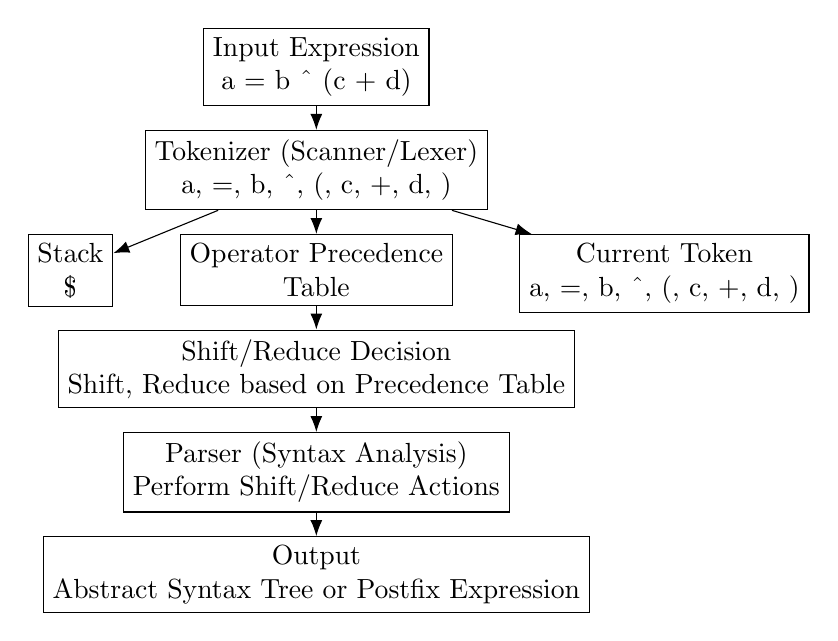
\begin{tikzpicture}[scale=0.2,  % 缩小整个图的比例
    node distance=0.3cm and 0.4cm,
    every node/.style={draw, align=center},
    arrow/.style={-{Latex[scale=1.2]}}
    ]

    \node (input) {Input Expression\\ a = b \textasciicircum\ (c + d)};
    \node (lexer) [below=of input] {Tokenizer (Scanner/Lexer)\\ a, =, b, \textasciicircum, (, c, +, d, )};
    \node (stack) [below left=of lexer] {Stack\\ \$};
    \node (token) [below right=of lexer] {Current Token\\ a, =, b, \textasciicircum, (, c, +, d, )};
    \node (table) [below=of lexer] {Operator Precedence\\ Table};
    \node (decision) [below=of table] {Shift/Reduce Decision\\ Shift, Reduce based on Precedence Table};
    \node (parser) [below=of decision] {Parser (Syntax Analysis)\\ Perform Shift/Reduce Actions};
    \node (output) [below=of parser] {Output\\ Abstract Syntax Tree or Postfix Expression};

    \draw [arrow] (input) -- (lexer);
    \draw [arrow] (lexer) -- (stack);
    \draw [arrow] (lexer) -- (token);
    \draw [arrow] (lexer) -- (table);
    \draw [arrow] (table) -- (decision);
    \draw [arrow] (decision) -- (parser);
    \draw [arrow] (parser) -- (output);

\end{tikzpicture}

算法如下:
\begin{algorithm}[H]
    \caption{Operator Precedence Parsing}
    \begin{algorithmic}[1]
        \State stack.push("\$")
        \While{true}
        \State top $\gets$ stack.top()
        \State lookahead $\gets$ input[0]
        \If{table[top][lookahead] == shift}
        \State shift()
        \State \textbf{continue}
        \ElsIf{table[top][lookahead] == reduce}
        \State reduce()
        \State \textbf{continue}
        \ElsIf{table[top][lookahead] == accept}
        \State accept()
        \State \textbf{return}
        \ElsIf{table[top][lookahead] == exception}
        \State throw exception()
        \EndIf
        \EndWhile
    \end{algorithmic}
\end{algorithm}
\newpage
\noindent
shift和reduce的算法如下:
\begin{algorithm}[H]
    \small
    \caption{Shift 操作}
    \begin{algorithmic}[1]
        \Function{shift}{}
        \State $stack.\text{push}(input[0])$
        \State $input.\text{erase}(0)$
        \EndFunction
    \end{algorithmic}
\end{algorithm}
\begin{figure}[H]
    \centering
    \includegraphics[width=0.6\linewidth]{shift.png}
    \caption{Paser->shift()}
    \label{fig:shift}
\end{figure}
\begin{algorithm}[H]
    \small
    \caption{Reduce 操作}
    \textcolor{red}{我们采用一个Reducer Class来进行规约操作,见\ref{ref:Parser}节}
    \begin{algorithmic}[1]
        \Function{reduce}{}
        \While{$table[stack.\text{top}()][input[0]] == \text{reduce}$}
        \State $result \gets \text{calculator}(stack)$
        \State $stack.\text{pop}()$
        \State $stack.\text{push}(result)$
        \EndWhile
        \EndFunction
    \end{algorithmic}
\end{algorithm}
\begin{figure}[H]
    \centering
    \includegraphics[width=0.6\linewidth]{reduce1.png}
    \caption{Paser->reduce()}
    \label{fig:reduce1}
\end{figure}
\begin{figure}[H]
    \centering
    \includegraphics[width=0.6\linewidth]{reuce2.png}
    \caption{Reducer->reduce()}
    \label{fig:reuce2}
\end{figure}


\newpage
\subsubsection{stack的说明}
我们对stack做如下的设计:
\begin{enumerate}
    \item \textbf{只处理终结符} 忽略非终结符可以简化对栈的操作。在规约操作中,只需要考虑终结符,可以更容易地进行计算和规约。
    \item \textbf{统一操作符行为}:通过明确每个操作符的行为,可以更方便地进行各种操作符的处理,提高算法的效率。
\end{enumerate}

\subsubsection{Parser(语法分析器)的实现}
Paser负责计算Token队列(过程中转为语法树),并检测语法错误.
Paser维护一个stack和一个输入buffer,并根据优先表进行shift和reduce操作(opp):
\paragraph{reduce 方法}
\texttt{reduce} 规约操作的角色,将表达式中的部分符号按照优先级进行计算

\paragraph{操作流程}
\begin{enumerate}
    \item 获取堆栈顶部的终结符和输入缓冲区中的第一个lookahead token。
    \item 在操作符优先级表中查找这两个token对应的动作。
    \item 如果这个动作指示进行规约(\texttt{action} 等于 1),那么我们就使用 \texttt{Reducer} 类对堆栈中的元素进行计算,并更新堆栈。这个过程会持续,直到不再需要规约
\end{enumerate}

\paragraph{shift 方法}
\texttt{shift} 方法用于将输入缓冲区中的token移入到堆栈中

\paragraph{操作流程}
\begin{enumerate}
    \item 根据lookahead token的类型,调用 \texttt{addInStack} 方法,将新的token对象加入栈。
    \item 然后token从输入缓冲区中移除
\end{enumerate}


\paragraph{opp 方法}
\texttt{opp} 方法是整个解析过程的核心,负责根据操作符的优先级决定是进行移入、规约或者返回最终计算结果。

\paragraph{操作流程}
\begin{enumerate}
    \item 在开始时,堆栈中会加入一个表示终止的分隔符 \texttt{"\$"}。
    \item 解析器会不断处理,直到整个表达式被解析完毕。具体步骤包括:
    \begin{enumerate}
        \item 获取当前堆栈顶部的终结符以及输入缓冲区中的lookahead token。
        \item 查找两者在优先级表中对应的动作 \texttt{action}。
        \item 根据 \texttt{action} 的值,执行相应的操作:
        \begin{itemize}
            \item 若为 \textbf{移入(0)}:执行 \texttt{shift},加入新的token。
            \item 若为 \textbf{规约(1)}:执行 \texttt{reduce},更新堆栈。
            \item 若为 \textbf{完成解析(2)}:调用 \texttt{getAnswer},返回计算结果。
            \item 若为 \textbf{异常情况(负数)}:根据错误类型抛出相应异常。
        \end{itemize}
    \end{enumerate}
\end{enumerate}
\label{ref:Parser}


\paragraph{表达式的计算 和 Reducer\\}
我们采用下表的规则进行reduce,注意上面的Token中只有decimal和boolean可能为non-terminal,所以\textcolor{red}{大体上}只有这两种Token可能会被reduce,其他Token只会被shift.

\begin{table}[H]
    \centering
    \small
    \begin{tabular}{|m{3.5cm}|m{3cm}|m{3cm}|m{5cm}|}
        \hline
        \textbf{输出类型}        & \textbf{操作}                                                        & \textbf{返回值}                   & \textbf{错误处理}                                                                              \\
        \hline
        Number/Boolean       & 无需操作                                                               & 该元素非终结符的恒等                     & 无                                                                                          \\
        \hline

        Unary Operators      & 弹出栈顶上的一个非终结符元素                                                     & 该元素取负或逻辑非后的副本                  & 如果栈顶上的元素缺失,报告缺失操作数错误;如果取负的元素不是数字或逻辑非的元素不是布尔值,报告类型不匹配错误                                     \\
        \hline
        Binary Operators & 弹出栈顶上下的一个非终结符元素                                                    & 对弹出元素进行运算的结果的副本                & 如果栈顶上下的元素缺失,报告缺失操作数错误;如果算术运算符和比较运算符用于非数字元素/逻辑运算符用于非布尔元素,报告类型不匹配错误                                \\
        \hline
        Ternary Operations   & 找到栈顶下方的第一个问号,提取问号前的元素作为A;提取问号后的元素作为B;提取冒号后的元素作为C                   & 如果A为真,返回B的非终结符副本;否则,返回C的非终结符副本 & 如果没有问号,报告三元运算符错误;如果问号和冒号之间的元素数量不是1,报告缺失操作符错误;如果A、B或C缺失或不是非终结符,报告缺失操作数错误;如果A不是布尔值,报告类型不匹配错误 \\
        \hline
        Parentheses          & 找到右括号下方的第一个左括号,提取括号之间的所有元素作为参数。如果左括号下方的元素为空或不是函数,执行常量操作;否则,执行函数操作。 & 常量操作无操作,函数操作对参数执行              & 如果常量操作的参数数量大于1,报告缺失操作符错误;如果参数为空或不是非终结符,报告缺失操作数错误;函数操作根据参数进行判断,一元函数通过方法判断,多参数函数要求参数交替为数字和逗号 \\
        \hline

        Others               & 无需操作                                                               & 无                              & 报告缺失操作符错误                                                                                  \\
        \hline
    \end{tabular}
\end{table}

\section{实验结果}
\subsection{新增测例说明}
\begin{itemize}
    \item \textbf{mytest.xml} 测试了所有的运算符,包括一元运算符,二元运算符,三元运算符,函数运算符,括号运算符,逗号运算符,终结符,非终结符,以及各种可能的异常情况.
    \item \textbf{mytest.bat} 用于运行mytest.xml
    \item \textbf{./src/paser/test} 是写代码时使用的Junit测试,里面加了几个调试过程中没有pass的测试用例,方便调试.
\end{itemize}
例如以下两个mytest.xml中的测例检测了文档中要求的\textcolor{red}{不区分大小写}和\textcolor{red}{函数缺少左括号应当抛出FunctionCallException}:
\begin{figure}[H]
    \centering
    \includegraphics[width=0.7\linewidth]{cases.png}
    \caption{test cases}
    \label{fig:cases}
\end{figure}
\newpage
\subsection{测试结果}
我的代码通过了所有能想到的测试用例:
\begin{figure}[htbp]
    \centering
    \begin{subfigure}[b]{0.5\textwidth}
        \centering
        \includegraphics[width=\linewidth]{simple.png}
        \caption{Simple}
        \label{fig:simple}
    \end{subfigure}
    %
    \begin{subfigure}[b]{0.5\textwidth}
        \centering
        \includegraphics[width=\linewidth]{standard.png}
        \caption{Standard}
        \label{fig:standard}
    \end{subfigure}
    
    \begin{subfigure}[b]{0.5\textwidth}
        \centering
        \includegraphics[width=\linewidth]{mytest.png}
        \caption{MyTest}
        \label{fig:mytest}
    \end{subfigure}
    \caption{Testing Results}
    \label{fig:combined}
\end{figure}
\newpage
\subsection{程序运行截图}
\begin{figure}[htbp]
    \centering
    \begin{subfigure}[b]{0.9\textwidth}
        \centering
        \includegraphics[width=\linewidth]{image24.png}
        \caption{RUN 1}
        \label{fig:image24}
    \end{subfigure}
    \hfill
    \begin{subfigure}[b]{0.9\textwidth}
        \centering
        \includegraphics[width=\linewidth]{image25.png}
        \caption{RUN 2}
        \label{fig:image25}
    \end{subfigure}
    
    \begin{subfigure}[b]{0.9\textwidth}
        \centering
        \includegraphics[width=\linewidth]{image26.png}
        \caption{RUN 3}
        \label{fig:image26}
    \end{subfigure}
    \hfill
    \begin{subfigure}[b]{0.9\textwidth}
        \centering
        \includegraphics[width=\linewidth]{image27.png}
        \caption{EXCEPTION 1}
        \label{fig:image27}
    \end{subfigure}
    
    \begin{subfigure}[b]{0.9\textwidth}
        \centering
        \includegraphics[width=\linewidth]{image28.png}
        \caption{EXCEPTION 2}
        \label{fig:image28}
    \end{subfigure}
    \hfill
    \begin{subfigure}[b]{0.9\textwidth}
        \centering
        \includegraphics[width=\linewidth]{image29.png}
        \caption{EXCEPTION 3}
        \label{fig:image29}
    \end{subfigure}
    
    \caption{Runs and Exceptions}
    \label{fig:combined}
\end{figure}
\section{心得体会}
\begin{itemize}
    \item \textbf{对于编译原理的理解} 通过这次实验,我对编译原理的一些基本概念有了更深的理解,如DFA,OPP,语法分析等,更深刻地认识到了如何处理各种特例中的细节.
    \item \textbf{对于Java的理解} 通过这次实验,我对Java的一些特性有了更深的理解,如接口,继承,多态等. 由于之前Java写得比较少,这次实验阅读了大量Java的文档,对Java的理解有了很大的提高.
    \item \textbf{对于代码的理解} 通过这次实验,我对代码的设计和实现有了更深的理解,如如何设计一个类,如何设计一个接口等.提高了我的软件工程水平.
\end{itemize}

\end{document}
